% \textbf{\underline{OZ 9 - Wisselstroomkringen - Oefening 1:}}
% \vspace{0.5cm}

% Beschouw een $ RLC $-circuit met in serie $ R = 150 \ \Omega $, $ L = 25,0 $ mH, en $ C = 2,00 \ \mu $F. Dit circuit wordt gevoed door een wisselspanningsbron met $ \Delta V_{rms} = 340 $ V en $ f = 660 $ Hz.

% \begin{enumerate}[(a)]
%     \item Bepaal de maximale stroom doorheen het circuit.
%     \item Bepaal de fasehoek tussen de stroom en de spanning over de bron.
%     \item Bepaal de maximale spanning over $ R $ en de fasehoek met de stroom.
%     \item Doe nu hetzelfde voor $ C $ en $ L $.
%     \item Teken het fasordiagram.
%     \item Maak een grafiek van de instantane stroom $ i $ en de instantane spanning $ \Delta v $ in functie van de tijd. Voeg ook de instantane spanning toe over de weerstand $ \Delta v_R $, de spoel $ \Delta v_L $ en de condensator $ \Delta v_C $.
%     \item Wat is het vermogen dat de bron levert aan de $ RLC $-kring?
%     \item Wat is de resonantiefrequentie van de $ RLC $-kring?
%     \item Als de bron wordt ingesteld op de resonantiefrequentie, wat is dan het vermogen dat de bron levert aan de $ RLC $-kring?
% \end{enumerate}

% \begin{description}[labelwidth=1.5cm, leftmargin=!]
%     \item[Geg. :]   $ R = 150 \ \Omega $; $ L = 25,0 $ mH; $ C = 2,00 \mu $F; $ \Delta V_{rms} = 340 $ V; $ f = 600 $ Hz;
% \end{description}

% \begin{enumerate}[(a)]
%     \item 
%         \begin{description}[labelwidth=1.5cm, leftmargin=!]
%             \item[Gevr. :]  $ I_{max} $;
%             \item[Opl. :]   $ X_L = \omega L 
%                             = 2 \pi f L 
%                             = 2\pi \cdot 660 \cdot 25,0 \cdot 10^{-3} 
%                             = 33 \pi \ \Omega $
            
%                             $ X_C = \dfrac{1}{\omega C} 
%                             = \dfrac{1}{2 \pi f C} 
%                             = \dfrac{1}{2 \pi \cdot 660 \cdot 2,00 \cdot 10^-6} 
%                             = \dfrac{1}{0,00264\pi} \ \Omega $
                            
%                             $ Z = \sqrt{R^2 + \left( X_L - X_C \right)^2} 
%                             = \sqrt{150^2 + \left( 33 \pi - \dfrac{1}{0,00264\pi} \right)^2} 
%                             = 150,9489605 \ \Omega $
                            
%                             $ I_{rms} = \dfrac{\Delta V_{rms}}{Z} 
%                             = \dfrac{340}{150,9489605} 
%                             = 2,252416968 $ A
                            
%                             $ I_{max} = \sqrt{2} I_{rms} 
%                             = \sqrt{2} \cdot 2,252416968 
%                             = 3,185398625 $ A $ 
%                             \approx 3,19 $ A
%         \end{description}
%     \item
%         \begin{description}[labelwidth=1.5cm, leftmargin=!]
%             \item[Gevr. :]  $ \phi $;
%             \item[Opl. :]   $ \phi = \tan^{-1}{\dfrac{X_L - X_C}{R}} 
%                             = \tan^{-1}{\dfrac{33 \pi - \dfrac{1}{0,00264\pi}}{150}} 
%                             = -6,427978507^{\circ} 
%                             \approx -6,43^{\circ} $
%         \end{description}
%     \item
%         \begin{description}[labelwidth=1.5cm, leftmargin=!]
%             \item[Gevr. :]  $ \Delta V_{R,max} $; $ \phi_R $;
%             \item[Opl. :]   $ \Delta V_{R,max} = I_{max} R 
%                             = 3,19 \cdot 150 
%                             = 478,5 $ V $ 
%                             \approx 479 $ V
                            
%                             $ \phi_R = 0^{\circ} $
%         \end{description}
%     \item
%         \begin{description}[labelwidth=1.5cm, leftmargin=!]
%             \item[Gevr. :]  $ \Delta V_{C,max} $; $ \phi_C $; $ \Delta V_{L,max} $; $ \phi_L $;
%             \item[Opl. :]   $ \Delta V_{C,max} = I_{max} X_C 
%                             = 3,19 \cdot \dfrac{1}{0,00264\pi} 
%                             = 384,624458 $ V $ 
%                             \approx 385 $ V
                            
%                             $ \phi_R = 90^{\circ} $
                            
%                             $ \Delta V_{L,max} = I_{max} X_L 
%                             = 3,19 \cdot 33 \pi 
%                             = 330,7154586 $ V $ 
%                             \approx 331 $ V
                            
%                             $ \phi_R = -90^{\circ} $
%         \end{description}
%     \item
%         \parbox{\linewidth}{
%             \centering
%             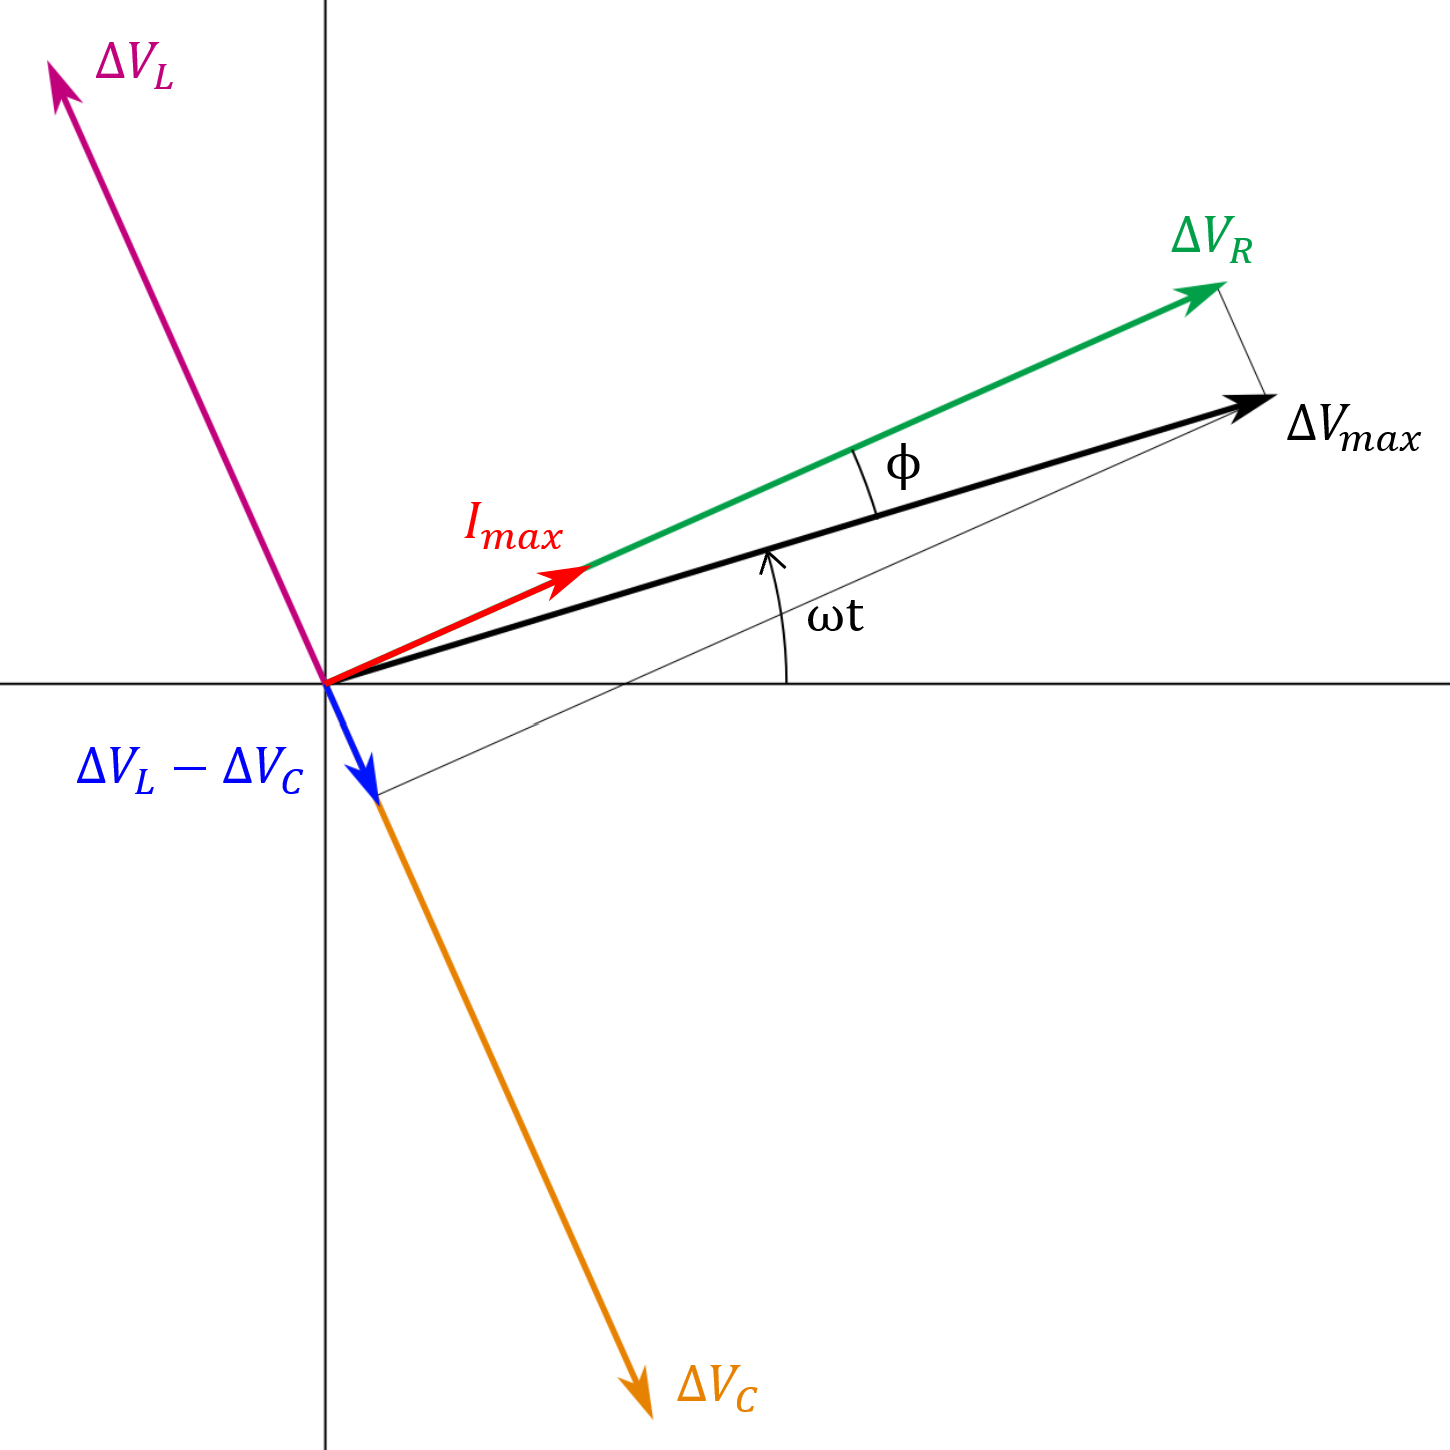
\includegraphics[width=8cm]{oz09/resources/oef-1-deelvraag-e.png}
%         }
%     \item
%         \parbox{\linewidth}{
%             \centering
%             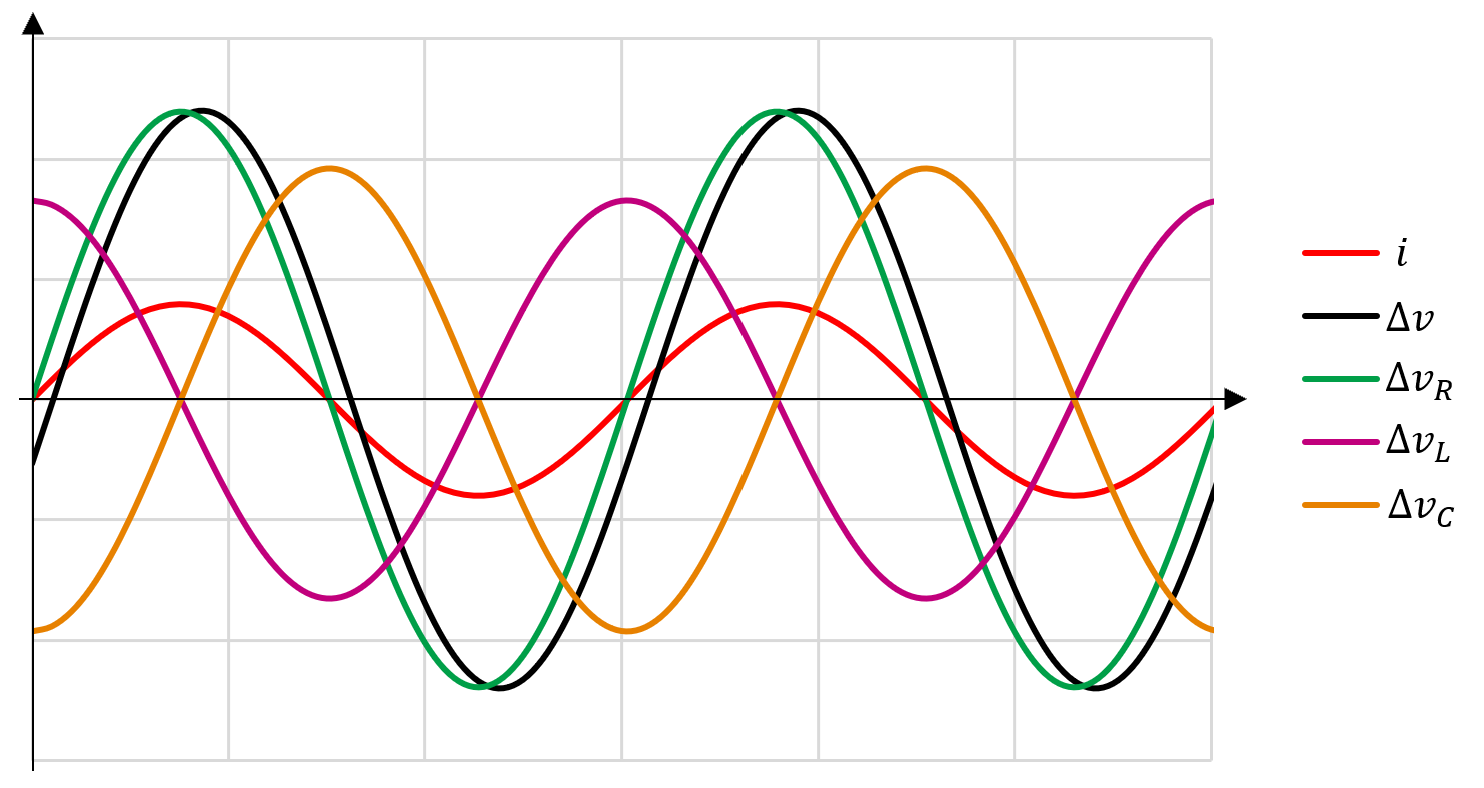
\includegraphics[width=12cm]{oz09/resources/oef-1-deelvraag-f.png}
%         }
%     \item
%         \begin{description}[labelwidth=1.5cm, leftmargin=!]
%             \item[Gevr. :]  $ P_{av} $;
%             \item[Opl. :]   $ P_{av} = I_{rms}^2 \cdot R 
%                             = 2,252416968^2 \cdot 150 
%                             = 761 $ W
%         \end{description}
%     \item
%         \begin{description}[labelwidth=1.5cm, leftmargin=!]
%             \item[Gevr. :]  $ f_0 $;
%             \item[Opl. :]   $ X_C = X_L $
            
%                             \hspace{-0.57cm} $ \Leftrightarrow 
%                             \dfrac{1}{\omega_0 C} = \omega_0 L $
            
%                             \hspace{-0.57cm} $ \Leftrightarrow 
%                             \dfrac{1}{2 \pi f_0 C} = 2 \pi f_0 L $
            
%                             \hspace{-0.57cm} $ \Leftrightarrow 
%                             \dfrac{1}{2 \pi f_0 C} = 2 \pi f_0 L $
            
%                             \hspace{-0.57cm} $ \Leftrightarrow 
%                             f_0 = \dfrac{1}{2 \pi \sqrt{L C}} 
%                             = \dfrac{1}{2 \pi \sqrt{25,0 \cdot 10^{-3} \cdot 2,00 \cdot 10^{-6}}} 
%                             = 711,7625434 $ Hz $ 
%                             \approx 712 $ Hz
%         \end{description}
%     \item
%         \begin{description}[labelwidth=1.5cm, leftmargin=!]
%             \item[Gevr. :]  $ P_{av} $ als $ f = f_0 $;
%             \item[Opl. :]   $ V_{R,rms} = V_{rms} $
            
%                             $ P_{av} = I_{rms} V_{R,rms} 
%                             = I_{rms} V_{rms} 
%                             = \dfrac{V_{rms}^2}{R} 
%                             = \dfrac{340^2}{150} 
%                             = 770,67 $ W $ 
%                             \approx 771 $ W
%         \end{description}
% \end{enumerate}

% \vspace{1cm}